\documentclass{beamer}

\usepackage[ruled]{algorithm2e}
\SetKw{KwRet}{return}
\usepackage{amsmath}

\usetheme{AnnArbor}
\usecolortheme{crane}
\usefonttheme[onlymath]{serif}

\title{Deep Learning - Foundations and Concepts}
\subtitle{Chapter 12. Transformers}
\author{nonlineark@github}
\date{\today}

\begin{document}

\begin{frame}
    \titlepage
\end{frame}

\begin{frame}
    \frametitle{Outline}
    \tableofcontents
\end{frame}

\section{Attention}

\begin{frame}
    \frametitle{Attention}
    The fundamental concept that underpins a transformer is attention:
    \begin{itemize}
        \item This was originally developed as an enhancement to RNNs for machine translation (\href{https://arxiv.org/abs/1409.0473}{Bahdanau, Cho and Bengio, 2014})
        \item Later, it was found that significantly improved performance could be obtained by eliminating the recurrence structure and instead focusing exclusively on the attention mechanism (\href{https://arxiv.org/abs/1706.03762}{Vaswani et al., 2017}).
    \end{itemize}
\end{frame}

\begin{frame}
    \frametitle{Attention}
    Consider the following two sentences:
    \begin{itemize}
        \item I swam across the river to get to the other bank.
        \item I walked across the road to get cash from the bank.
    \end{itemize}
    Here the word ``bank'' has different meanings in the two sentences:
    \begin{itemize}
        \item In the first sentence, the words ``swam'' and ``river'' most strongly indicate that ``bank'' refers to the side of a river.
        \item In the second sentence, the word ``cash'' is a strong indicator that ``bank'' refers to a financial institution.
    \end{itemize}
    To determine the appropriate interpretation of ``bank'', a neural network processing such a sentence should:
    \begin{itemize}
        \item Attend to specific words from the rest of the sequence.
        \item The particular locations that should receive more attention depend on the input sequence itself.
    \end{itemize}
\end{frame}

\begin{frame}
    \frametitle{Transformer processing}
    \begin{itemize}
        \item The input data to a transformer is a set of vectors $\{x_{n}\}$ of dimensionality $D$, where $n=1,\hdots,N$.
        \item We refer to these data vectors as tokens, and the elements of the tokens are called features.
        \item We will combine the tokens into a matrix $X$ of dimension $N\times{}D$ in which the $n$th row comprises the token $x_{n}^{T}$.
    \end{itemize}
    \begin{figure}
        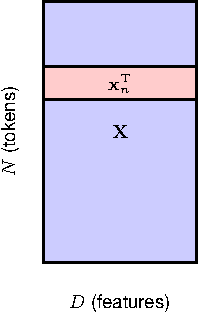
\includegraphics[height=0.4\textheight]{Figure_3.pdf}
    \end{figure}
\end{frame}

\begin{frame}
    \frametitle{Transformer processing}
    The fundamental building block of a transformer is a function that takes a data matrix $X$ as input and creates a transformed matrix $\tilde{X}$ of the same dimensionality as the output:
    \begin{equation*}
        \tilde{X}=\mathrm{TransformerLayer}(X)
    \end{equation*}
    A single transformer layer itself comprises two stages:
    \begin{itemize}
        \item The first stage, which implements the attention mechanism, mixes together the corresponding features from different tokens across the columns of the data matrix.
        \item The second stage acts on each row independently and transforms the features within each token.
    \end{itemize}
\end{frame}

\begin{frame}
    \frametitle{Attention coefficients}
    Suppose we have a set of input tokens $x_{1},\hdots,x_{N}$ and we want to map this set to another set $y_{1},\hdots,y_{N}$:
    \begin{itemize}
        \item $y_{n}$ should depend on all the tokens $x_{1},\hdots,x_{N}$.
        \item This dependence should be stronger for those tokens $x_{m}$ that are particularly important for determining the modified representation of $y_{n}$.
    \end{itemize}
    A simple way to achieve this is to define each output token $y_{n}$ to be a linear combination of the input tokens:
    \begin{align*}
        y_{n}&=\sum_{m=1}^{N}a_{nm}x_{m} \\
        a_{nm}&\ge{}0\qquad\sum_{m=1}^{N}a_{nm}=1
    \end{align*}
\end{frame}

\begin{frame}
    \frametitle{Self-attention}
    The problem of determining the attention coefficients can be viewed from an information retrieval perspective:
    \begin{itemize}
        \item We could view the vector $x_{n}$ as:
        \begin{itemize}
            \item The key for input token $n$.
            \item The value for input token $n$.
            \item The query for output token $n$.
        \end{itemize}
        \item To measure the similarity between the query $x_{n}$ and the key $x_{m}$, we could use their dot product: $x_{n}^{T}x_{m}$.
        \item To make sure the attention coefficients define a partition of unity, we could use the $\mathrm{softmax}$ function to transform the dot products.
    \end{itemize}
\end{frame}

\begin{frame}
    \frametitle{Self-attention}
    Dot-product self-attention:
    \begin{align*}
        y_{n}&=\sum_{m=1}^{N}a_{nm}x_{m} \\
        a_{nm}&=\frac{\exp(x_{n}^{T}x_{m})}{\sum_{m'=1}^{N}\exp(x_{n}^{T}x_{m'})}
    \end{align*}
    Or write in matrix notation:
    \begin{equation*}
        Y=\mathrm{softmax}(XX^{T})X
    \end{equation*}
    where $\mathrm{softmax}(L)$ means to apply $\mathrm{softmax}$ to each row of the matrix $L$.
\end{frame}

\begin{frame}
    \frametitle{Network parameters}
    The current transformation from input tokens $\{x_{n}\}$ to output tokens $\{y_{n}\}$ has major limitations:
    \begin{itemize}
        \item The transformation is fixed and has no capacity to learn from data because it has no adjustable parameters.
        \item Each of the feature values within a token $x_{n}$ plays an equal role in determining the attention coefficients.
    \end{itemize}
\end{frame}

\begin{frame}
    \frametitle{Network parameters}
    We can overcome these limitations by defining separate query, key and value matrices each having their own independent linear transformations:
    \begin{itemize}
        \item $Q=XW^{(q)}$, where $W^{(q)}$ has dimensionality $N\times{}D_{k}$.
        \item $K=XW^{(k)}$, where $W^{(k)}$ has dimensionality $N\times{}D_{k}$.
        \item $V=XW^{(v)}$, where $W^{(v)}$ has dimensionality $N\times{}D_{v}$.
        \item A typical choice is $D_{k}=D$.
        \item If we set $D_{v}=D$:
        \begin{itemize}
            \item This will facilitate the inclusion of residual connections.
            \item Multiple transformer layers can be stacked on top of each other.
        \end{itemize}
    \end{itemize}
    The dot-product self-attention now takes the form:
    \begin{equation*}
        Y=\mathrm{softmax}(QK^{T})V
    \end{equation*}
\end{frame}

\begin{frame}
    \frametitle{Scaled self-attention}
    \begin{itemize}
        \item When logits are too large, the $\mathrm{softmax}$ function will produce extremely small gradients, which is not desirable.
        \item We need to scale the logits before applying the $\mathrm{softmax}$ function.
        \item Notice that if $q,k\in\mathbb{R}^{D_{k}}$ and the elements of $q$ and $k$ are all independent random numbers with zero mean and unit variance, then $\mathrm{var}(q^{T}k)=D_{k}$. Thus it would be appropriate to scale the logits by the standard deviation $\sqrt{D_{k}}$.
    \end{itemize}
    The scaled dot-product self-attention now takes the form:
    \begin{equation*}
        Y=\mathrm{Attention}(Q,K,V)=\mathrm{softmax}(\frac{QK^{T}}{\sqrt{D_{k}}})V
    \end{equation*}
\end{frame}

\begin{frame}
    \frametitle{Scaled self-attention}
    \begin{figure}
        \caption{Information flow in a scaled dot-product self-attention neural network layer}
        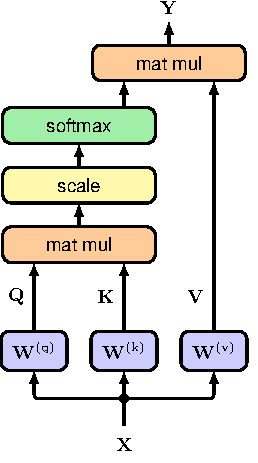
\includegraphics[height=0.7\textheight]{Figure_6.pdf}
    \end{figure}
\end{frame}

\begin{frame}
    \frametitle{Scaled self-attention}
    \begin{algorithm}[H]
        \caption{Scaled dot-product self-attention}
        $Q\gets{}XW^{(q)}$\;
        $K\gets{}XW^{(k)}$\;
        $V\gets{}XW^{(v)}$\;
        \Return{$\mathrm{Attention}(Q,K,V)=\mathrm{softmax}(\frac{QK^{T}}{\sqrt{D_{k}}})V$}\;
    \end{algorithm}
\end{frame}

\begin{frame}
    \frametitle{Multi-head attention}
    We can use multiple attention heads in parallel to attend to multiple data-dependent patterns at the same time. Suppose we have $C$ heads:
    \begin{align*}
        H_{c}&=\mathrm{Attention}(Q_{c},K_{c},V_{c}) \\
        &=\mathrm{Attention}(XW^{(q)}_{c},XW^{(k)}_{c},XW^{(v)}_{c})
    \end{align*}
    The heads are first concatenated into a single matrix, and the result is then linearly transformed using a matrix $W^{(o)}$ to give a combined output:
    \begin{equation*}
        Y=(H_{1},\hdots,H_{C})W^{(o)}
    \end{equation*}
    The matrix $W^{(o)}$ has dimension $HD_{v}\times{}D$, so that the final output matrix $Y$ has dimension $N\times{}D$.
\end{frame}

\begin{frame}
    \frametitle{Multi-head attention}
    \begin{figure}
        \caption{Information flow in a multi-head attention layer}
        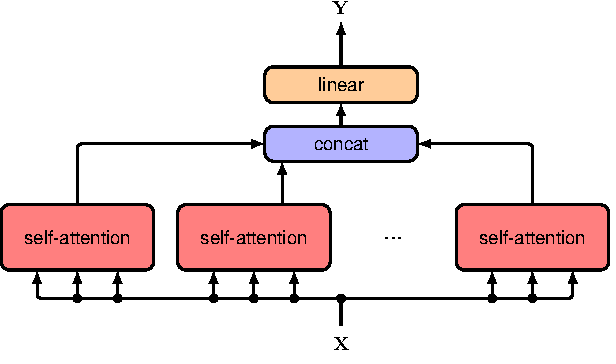
\includegraphics[height=0.7\textheight]{Figure_8.pdf}
    \end{figure}
\end{frame}

\begin{frame}
    \frametitle{Multi-head attention}
    \begin{algorithm}[H]
        \caption{Multi-head attention}
        \For{$c\gets{}1$ \KwTo $C$}{
            $Q_{c}=XW^{(q)}_{c}$\;
            $K_{c}=XW^{(k)}_{c}$\;
            $V_{c}=XW^{(v)}_{c}$\;
            $H_{c}=\mathrm{Attention}(Q_{c},K_{c},V_{c})$\;
        }
        $H=(H_{1},\hdots,H_{C})$\;
        \Return{$Y=HW^{(o)}$}\;
    \end{algorithm}
\end{frame}

\begin{frame}
    \frametitle{Transformer layers}
    To improve training efficiency, we can introduce residual connections and layer normalization:
    \begin{equation*}
        Z=\mathrm{LayerNorm}(Y(X)+X)
    \end{equation*}
    Or using pre-norm:
    \begin{equation*}
        Z=Y(\mathrm{LayerNorm}(X))+X
    \end{equation*}
    Until now, the output data matrix $Y$ is still a linear transformation of the input data matrix $X$, and this limits the expressive capabilities of the attention layer. We can enhance the flexibility by post-processing the outputs using a standard nonlinear neural network denoted $\mathrm{MLP}$:
    \begin{equation*}
        \tilde{X}=\mathrm{LayerNorm}(\mathrm{MLP}(Z)+Z)
    \end{equation*}
    Again, we can use a pre-norm instead:
    \begin{equation*}
        \tilde{X}=\mathrm{MLP}(\mathrm{LayerNorm}(Z))+Z
    \end{equation*}
\end{frame}

\begin{frame}
    \frametitle{Transformer layers}
    \begin{figure}
        \caption{One layer of the transformer architecture}
        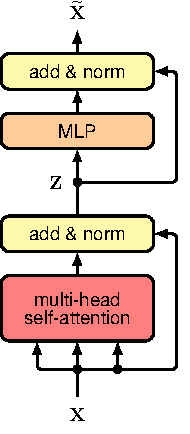
\includegraphics[height=0.7\textheight]{Figure_9.pdf}
    \end{figure}
\end{frame}

\begin{frame}
    \frametitle{Computational complexity}
    \begin{itemize}
        \item In the attention layer:
        \begin{itemize}
            \item Calculate the matrices $Q$, $K$ and $V$: $\mathcal{O}(ND^{2})$.
            \item Calculate the dot products $QK^{T}$: $\mathcal{O}(N^{2}D)$.
            \item Calculate the matrix $Y$: $\mathcal{O}(N^{2}D)$.
        \end{itemize}
        \item In the neural network layer:
        \begin{itemize}
            \item Calculate the matrix $\tilde{X}$: $\mathcal{O}(ND^{2})$.
        \end{itemize}
    \end{itemize}
\end{frame}

\begin{frame}
    \frametitle{Positional encoding}
    \begin{itemize}
        \item A transformer is equivariant with respect to input permutations due to the shared matrices $W^{(q)}_{c}$, $W^{(k)}_{c}$, $W^{(v)}_{c}$ and the shared subsequent neural network.
        \item The lack of dependence on token order becomes a major limitation when we consider sequential data, so we need to find a way to inject token order information into the network.
    \end{itemize}
\end{frame}

\begin{frame}
    \frametitle{Positional encoding}
    The requirements for a positional encoding:
    \begin{itemize}
        \item The token order should be encoded in the data itself instead of having to be represented in the network architecture.
        \item We will construct a position encoding vector $r_{n}$ associated with each input position $n$ and then combine this with the associated input token $x_{n}$:
        \begin{itemize}
            \item {[No]} $\tilde{x}_{n}=(x_{n},r_{n})$.
            \item {[Yes]} $\tilde{x}_{n}=x_{n}+r_{n}$.
        \end{itemize}
        \item $r_{n}$ should be bounded.
        \item $r_{n}$ should generalize well to new input sequences that are longer than those used in training.
        \item $r_{n}$ should be unique for a given position.
        \item $r_{n}$ should have a consistent way to express the number of steps between any two input tokens irrespective of their absolute position.
    \end{itemize}
\end{frame}

\begin{frame}
    \frametitle{Positional encoding}
    Positional encoding based on sinusoidal functions:
    \begin{align*}
        r_{ni}=\begin{cases}
            \sin(\frac{n}{L^{\frac{i}{D}}}),\textrm{if $i$ is even} \\
            \cos(\frac{n}{L^{\frac{i-1}{D}}}),\textrm{if $i$ is odd}
        \end{cases}
    \end{align*}
    \begin{figure}
        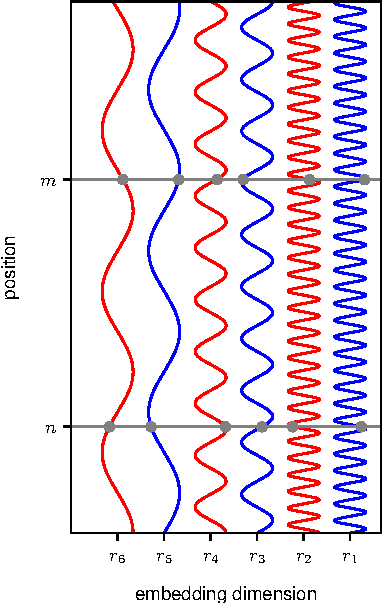
\includegraphics[height=0.5\textheight]{Figure_10_a.pdf}
    \end{figure}
\end{frame}

\end{document}